\begin{figure}[ht]
\centering
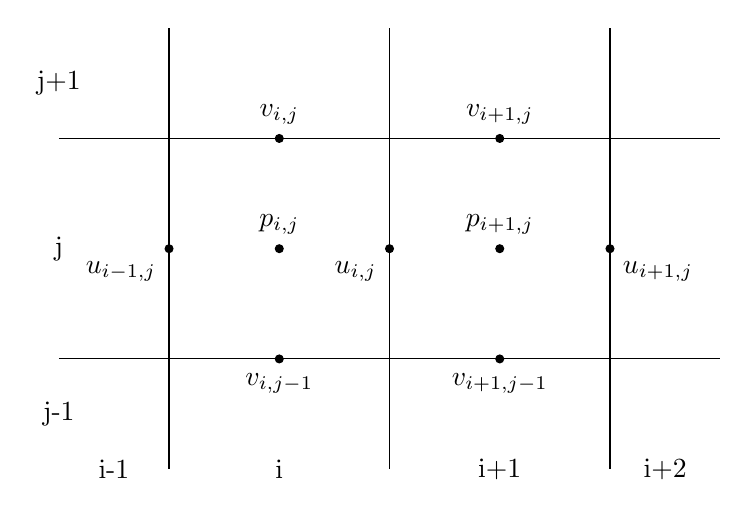
\begin{tikzpicture}[scale=1.4]

\draw (0, 1) -- (6, 1);
\draw (0, 3) -- (6, 3);

\draw (1,4) -- (1,0);
\draw (3,4) -- (3,0);
\draw (5,4) -- (5,0);

\node at (0, 0.5) {j-1}; 
\node at (0, 2) {j}; 
\node at (0, 3.5) {j+1};

\node at (0.5, 0) {i-1}; 
\node at (2, 0) {i}; 
\node at (4, 0) {i+1};
\node at (5.5, 0) {i+2};

\node[label=above:{$p_{i,j}$}, draw, circle, fill, minimum size=0.1cm, inner sep=0pt] at (2, 2) {};
\node[label=above:{$p_{i+1,j}$}, draw, circle, fill, minimum size=0.1cm, inner sep=0pt] at (4, 2) {};

\node[label=below left:{$u_{i-1,j}$}, draw, circle, fill, minimum size=0.1cm, inner sep=0pt] at (1, 2) {};
\node[label=below left:{$u_{i,j}$}, draw, circle, fill, minimum size=0.1cm, inner sep=0pt] at (3, 2) {};
\node[label=below right:{$u_{i+1,j}$}, draw, circle, fill, minimum size=0.1cm, inner sep=0pt] at (5, 2) {};

\node[label=above:{$v_{i,j}$}, draw, circle, fill, minimum size=0.1cm, inner sep=0pt] at (2, 3) {};
\node[label=above:{$v_{i+1,j}$}, draw, circle, fill, minimum size=0.1cm, inner sep=0pt] at (4, 3) {};

\node[label=below:{$v_{i,j-1}$}, draw, circle, fill, minimum size=0.1cm, inner sep=0pt] at (2, 1) {};
\node[label=below:{$v_{i+1,j-1}$}, draw, circle, fill, minimum size=0.1cm, inner sep=0pt] at (4, 1) {};

\end{tikzpicture}
    \caption{Discretization points for each variable on the staggered grid\cite{book:griebel1998numerical}}
    \label{fig:staggered_grid}
\end{figure}